\chapter{Projeto Conceitual}


\section{Requisitos}
\label{requisitos}
	
Durante o desenvolvimento do projeto, foram priorizadas algumas características em detrimento de outras visando otimizar a missão definida para a aeronave.
Para isso, foi desenvolvida uma lista de prioridades que serão seguidas visando direcionar o desenvolvimento do projeto de maneira mais clara. 
	
Como se trata de uma aeronave que fará o transporte de pessoas, o projeto deve priorizar a segurança dos tripulantes e ocupantes em caso de acidentes, tendo boas configurações em caso de impacto e pouso brusco.
O projeto deve ser feito visando diminuir ao máximo a probabilidade de ocorrer um eventual incidente, sendo, portanto, a segurança operacional a primeira prioridade.

Sabe-se que o mercado no qual a aeronave estará atuando é o de voos regionais de companhias aéreas caracterizadas como “low-cost”, portanto, o fator mais atraente para uma aeronave sob esse ponto de vista é o baixo custo operacional.
Estabeleceu-se como prioridade número dois para o projeto, o desenvolvimento de uma aeronave com ótimo desempenho, devido à essa demanda especifica do público alvo.

Visando obter um ótimo desempenho, portanto, vê-se como terceira prioridade reduzir o peso estrutural da aeronave, visto que isto influencia fortemente no desempenho da aeronave e consequentemente no custo de operação.
Como quarta prioridade, com a finalidade de diminuir o custo final de aquisição da aeronave, tem-se a facilidade construtiva, e sempre que possível serão realizadas análises representativas e seguras visando reduzir o custo de engenharia.

Sabendo-se que o principal mercado que essa aeronave atuará é de voos definidos como \emph{short-haul}, isto é, voos de até 3 horas.
Apenas um conforto mínimo é requerido pelos passageiros, logo a ergonomia interna da aeronave é definida como quinta prioridade do projeto.
Um conforto dos passageiros melhor do que das principais aeronaves competidoras do mercado é um aspecto relativamente determinante na concepção interna do avião, visto que uma melhoria da ergonomia faz com que a aeronave se torne mais atraente no mercado se comparada às concorrentes.

Pelo fato de se tratar de uma aeronave de transporte de passageiros, com a missão de traslado, a aeronave não exige movimentos abruptos, com exceção de situações emergenciais que serão analisadas conforme regulamento.
Portanto, a manobrabilidade não é um item prioritário no desenvolvimento do projeto, sendo classificada como a sétima prioridade de projeto, logo após a estabilidade.
Portanto, o desenvolvimento do projeto da aeronave seguirá a ordem de prioridades conforme descrito na tabela abaixo. 

\begin{enumerate}
  \item \textbf{Segurança operacional:} avaliar a segurança da aeronave em todos os aspectos;
  \item \textbf{Desempenho:} escolher um grupo moto propulsor que atenda a missão e tenha baixo consumo, otimizar a aerodinâmica da aeronave reduzindo o arrasto, e portanto, reduzir do custo operacional;
  \item \textbf{Peso Estrutural:} reduzir o peso estrutural, visando melhor desempenho da aeronave;
  \item \textbf{Custo Final:} incluir processos de fabricação mais simples e sempre que possível reduzir os custos de engenharia, realizando análises representativas e seguras;
  \item \textbf{Ergonomia Interna:} avaliar o conforto do passageiro em todos os aspectos; 
  \item \textbf{Estabilidade:} proporcionar maior conforto durante o voo, aumentando a resistência da aeronave a fatores desestabilizandes (como rajadas e turbulências);
  \item \textbf{Manobrabilidade:} garantir a aeronavegabilidade da aeronave atendendo os requisitos da norma. 
\end{enumerate}
    
\section{Esboço do avião}
\label{esbocoinicial}
\subsection{Geometria Externa}
Duas propostas preliminares de configuração externa foram definidas por este estudo inicial, a saber 
\begin{description}
\item[Turbo-hélice] com asa alta otimizada para melhorar a influência do escoamento da hélice na asa de forma a maximizar L/D, motores abaixo da asa e empenagem em T, muito similar aos turboprops dessa capacidade existentes no mercado, ATR~42 e Bombardier Dash~8, \autoref{fig:turbo-helice};
\item[Turbofan/propfan com enflexamento negativo,] asa baixa e motores na configuração \emph{pusher}, próximos à cauda em T, \autoref{fig:propfan}.
\end{description}

\begin{figure}[H]
\centering
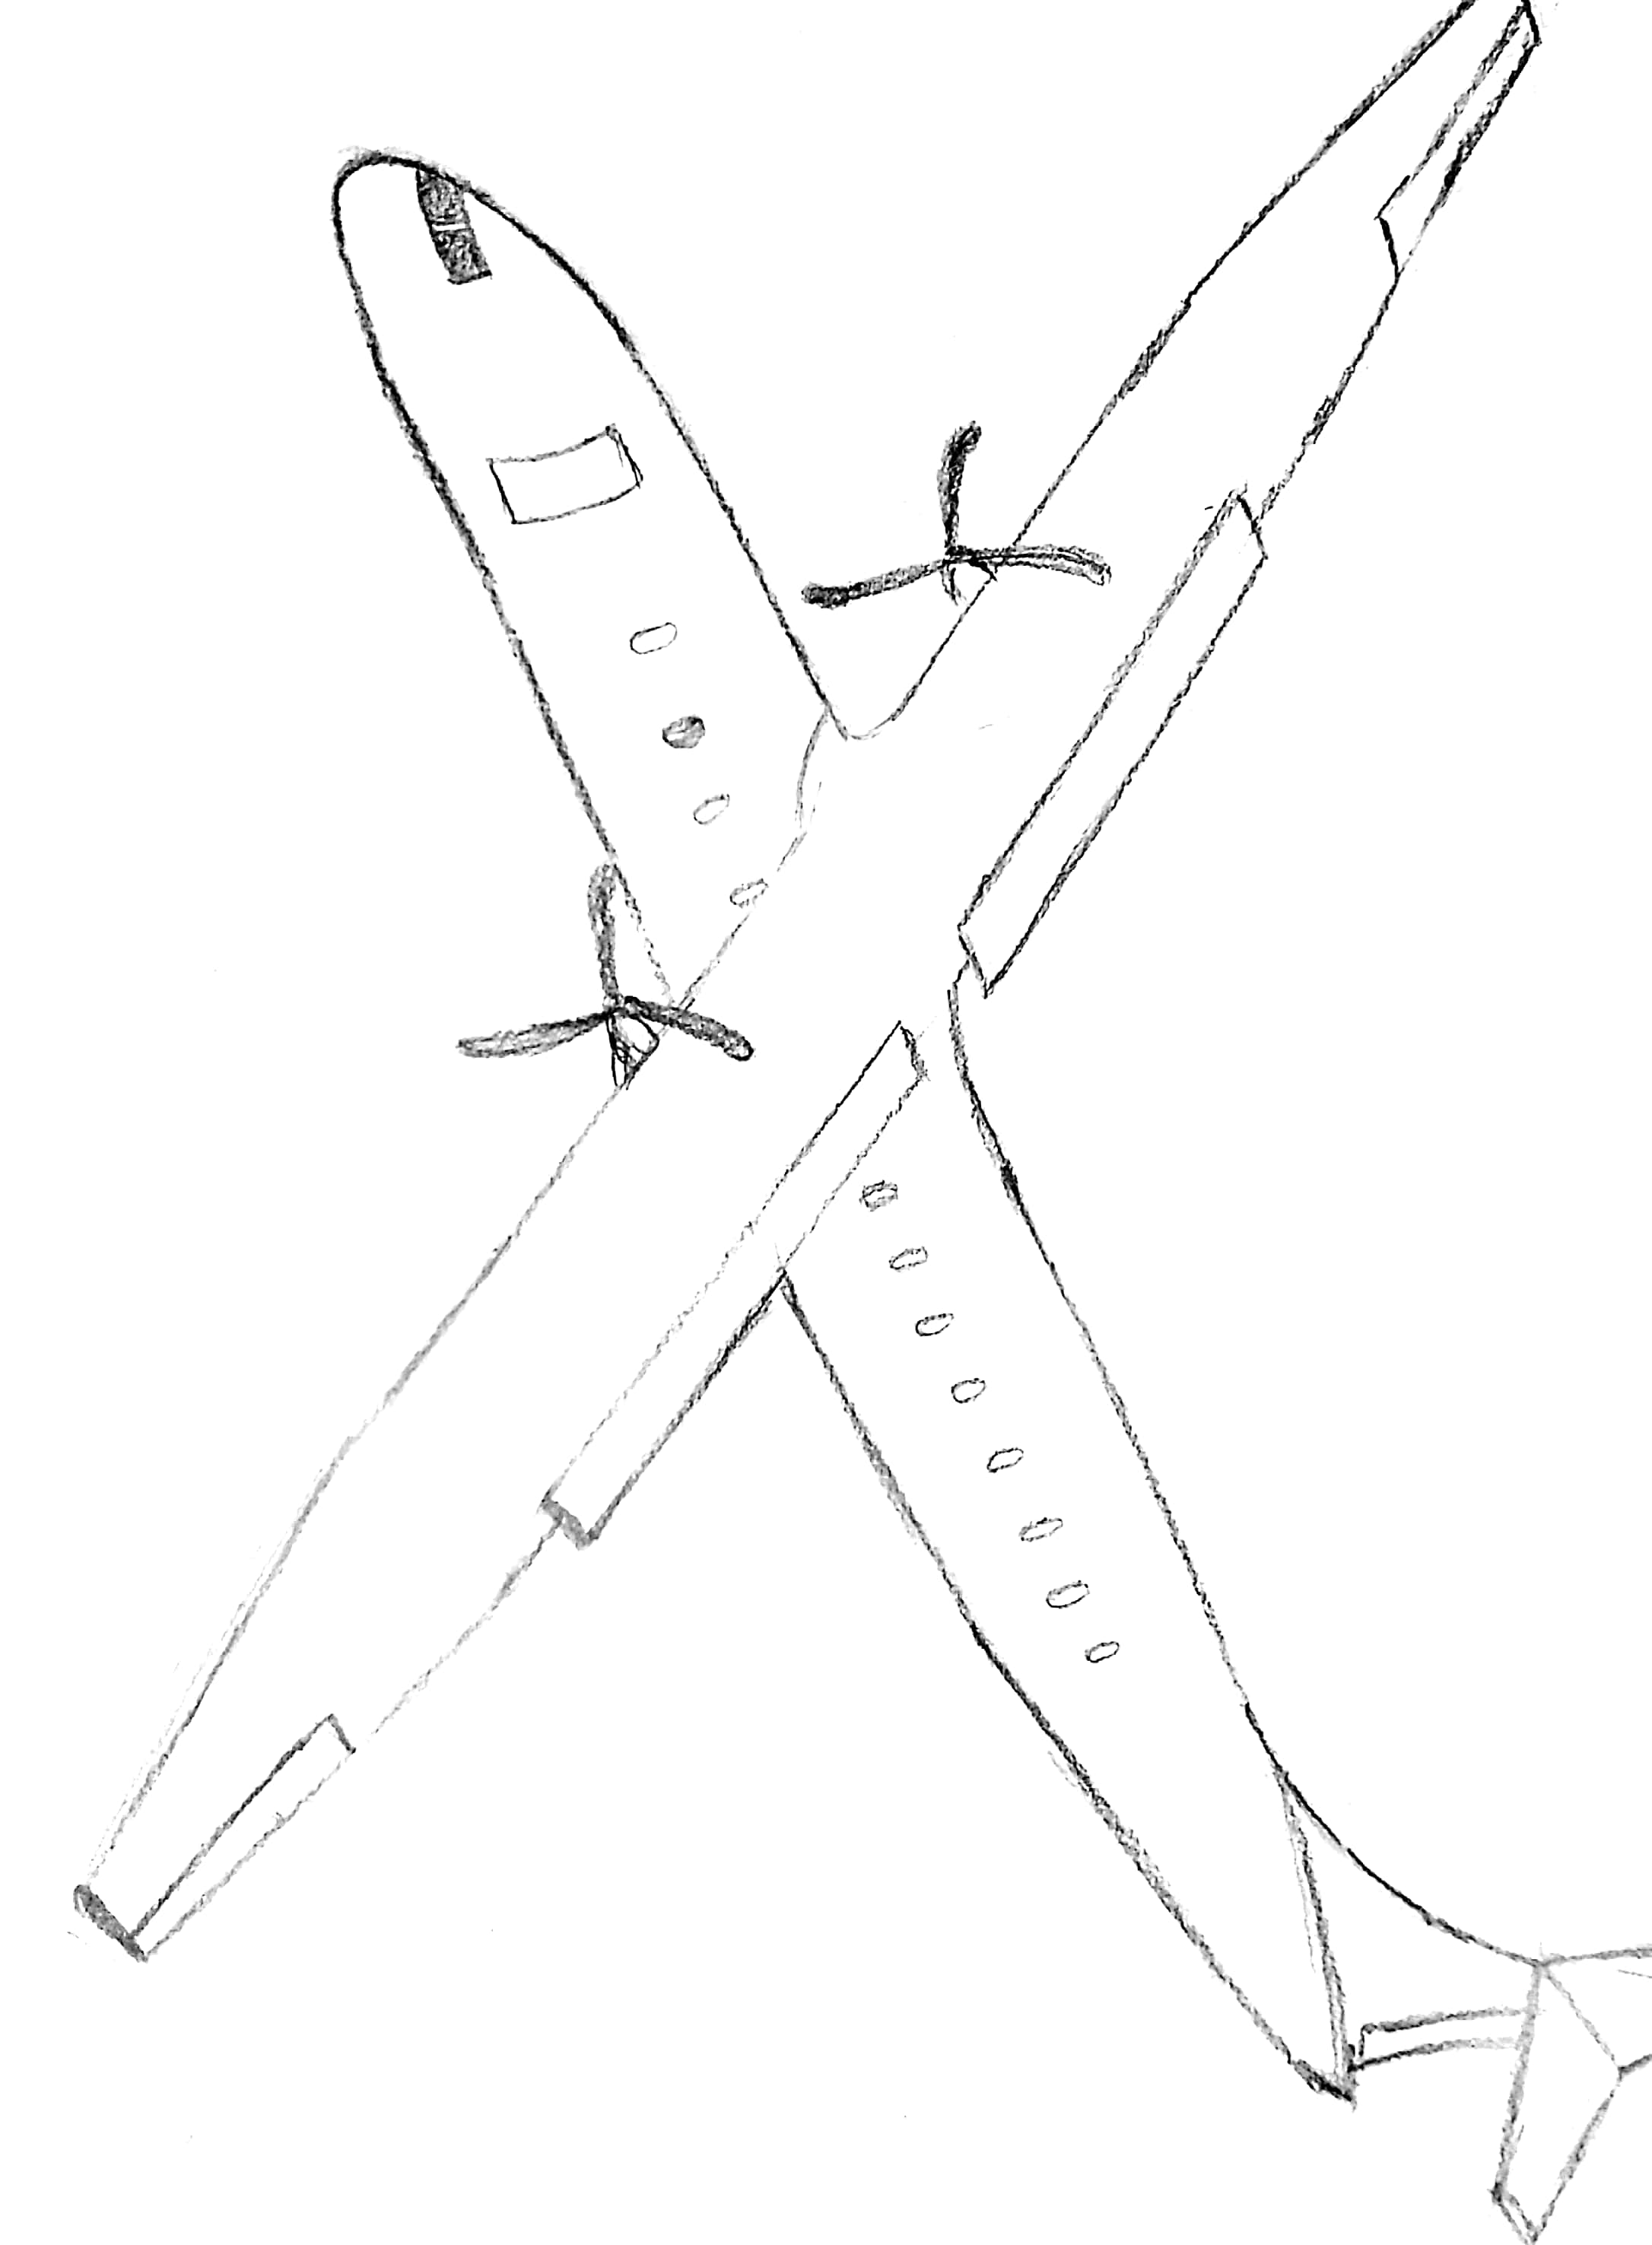
\includegraphics[width=0.5\textwidth,angle=90]{Modelos_Projetos_1_2.jpg}
\caption{Conceito de um turbo-hélice}
\label{fig:turbo-helice}
\end{figure}

\begin{figure}[H]
\centering
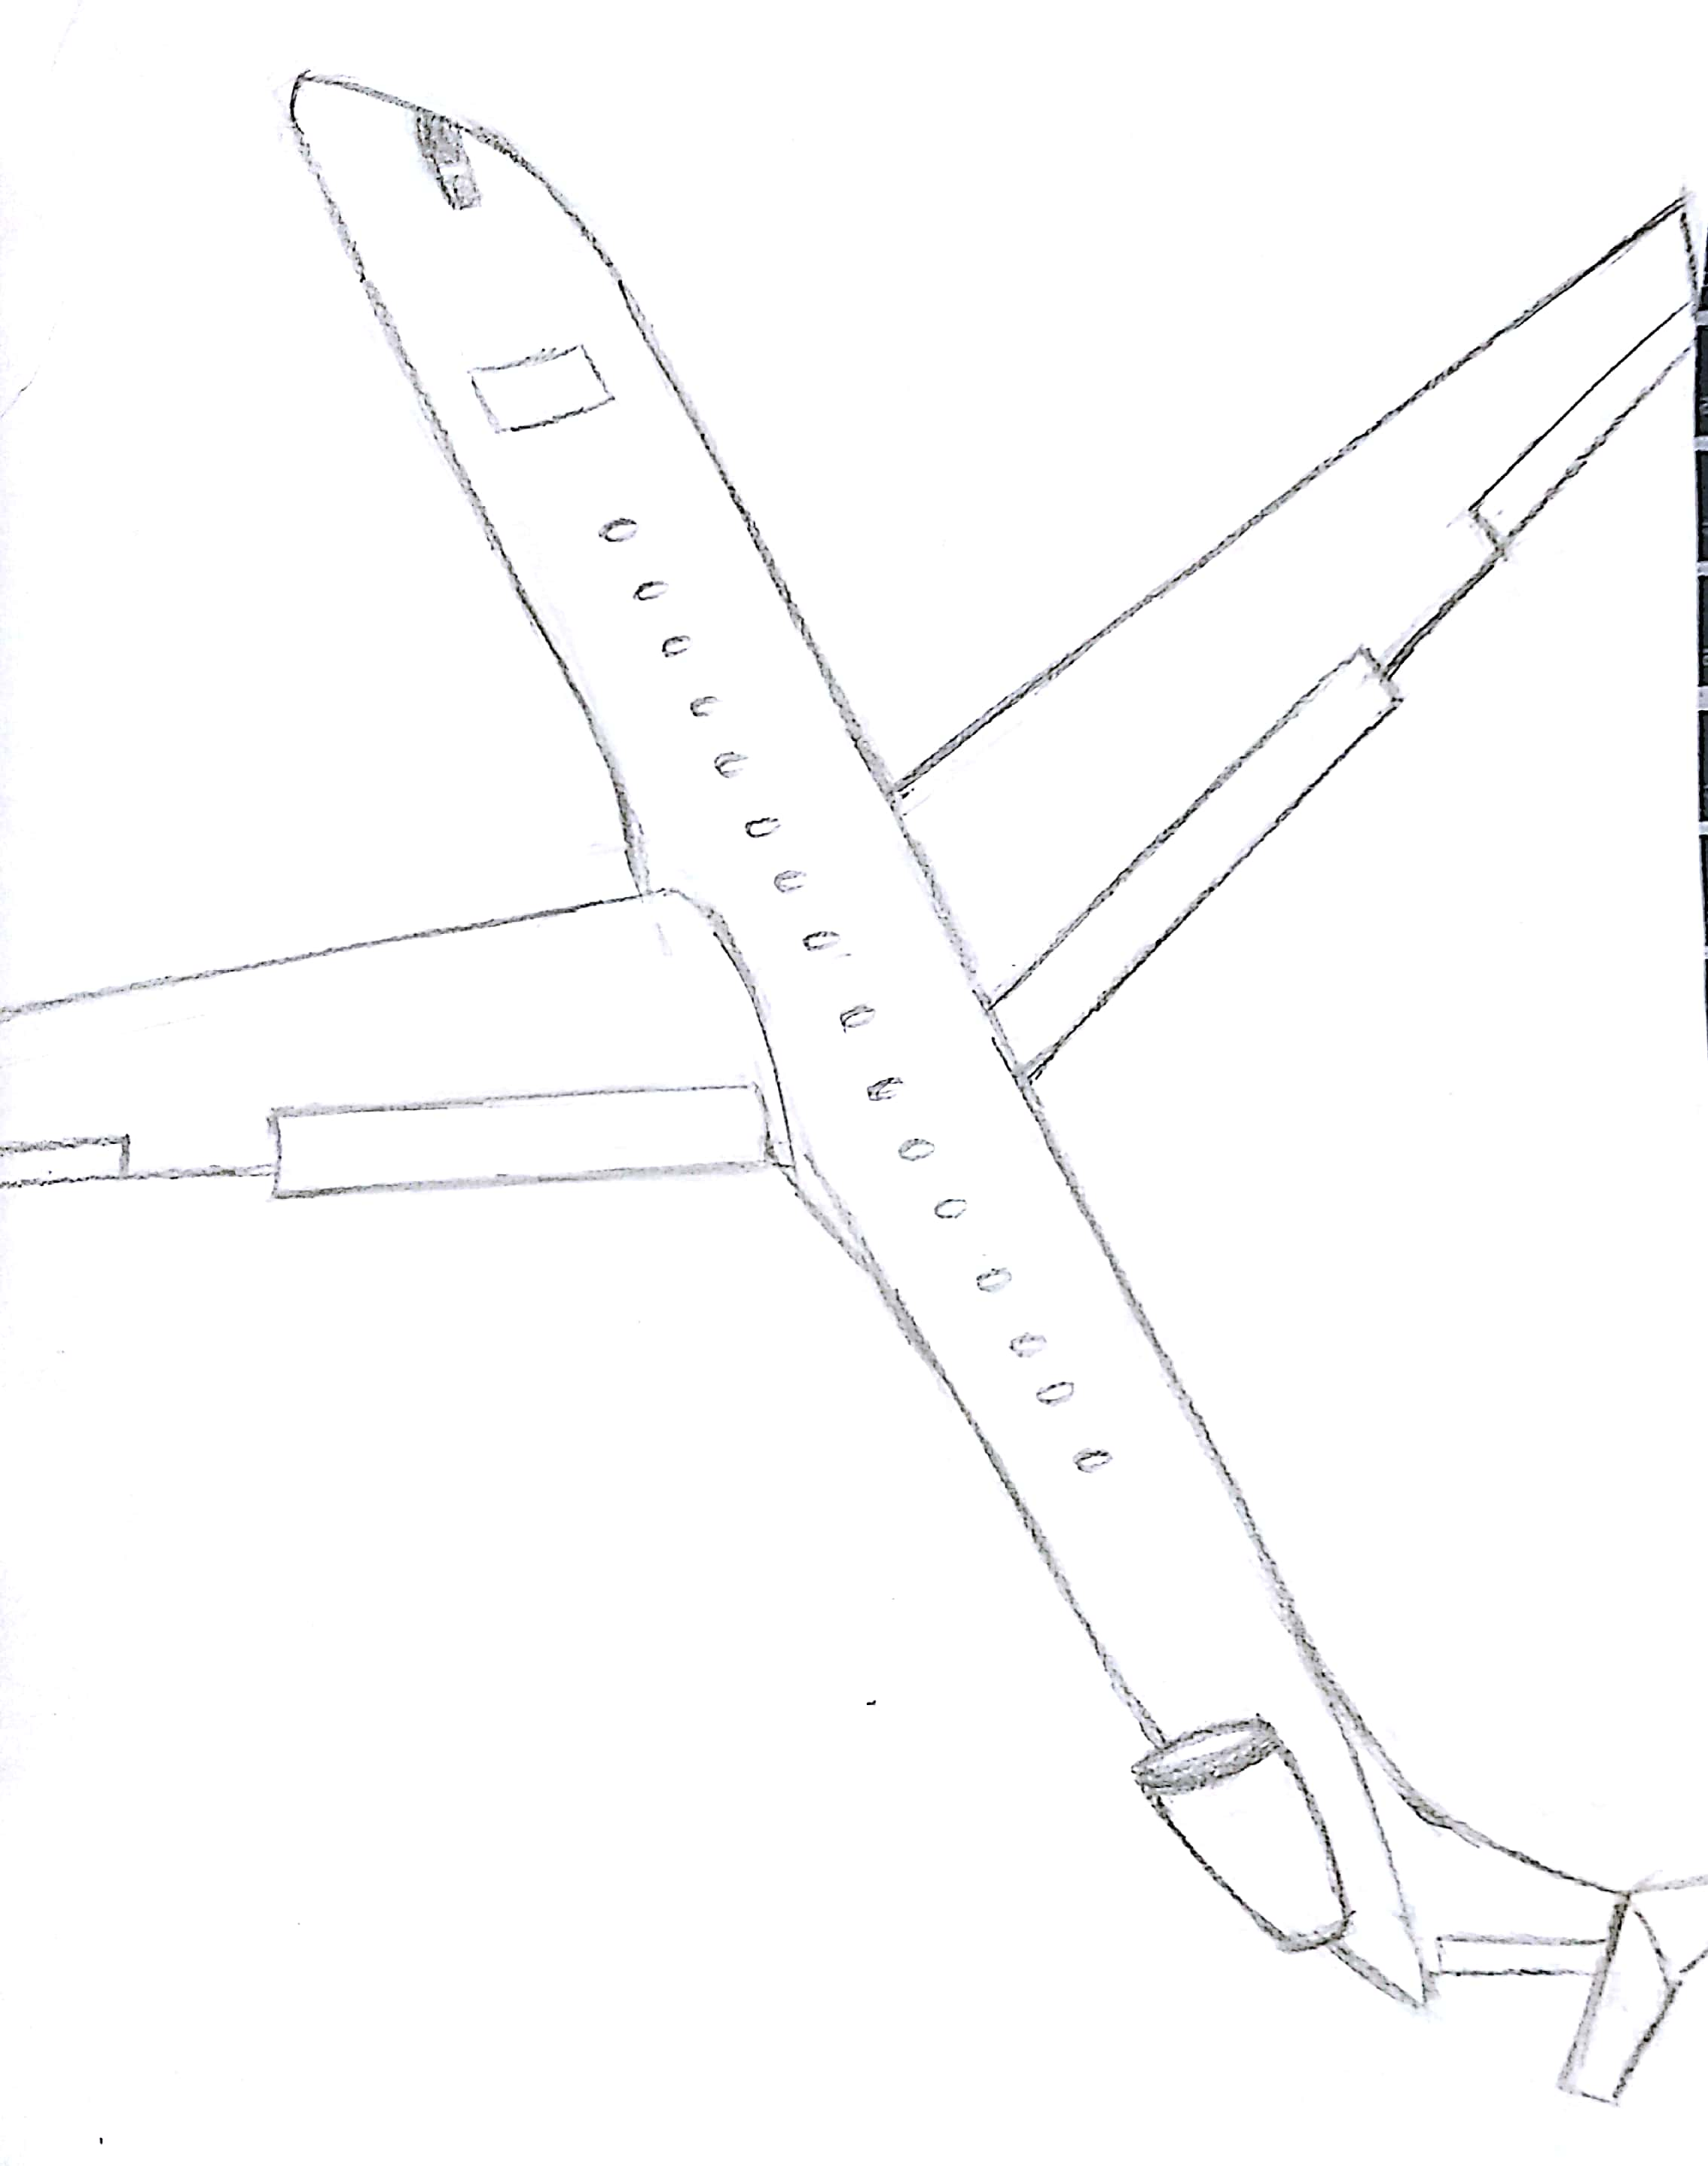
\includegraphics[width=0.5\textwidth,angle=90]{Modelos_Projetos_1_1.jpg}
\caption{Conceito de um turbofan/propfan com enflechamento negativo}
\label{fig:propfan}
\end{figure}

\begin{figure}[H]
\centering
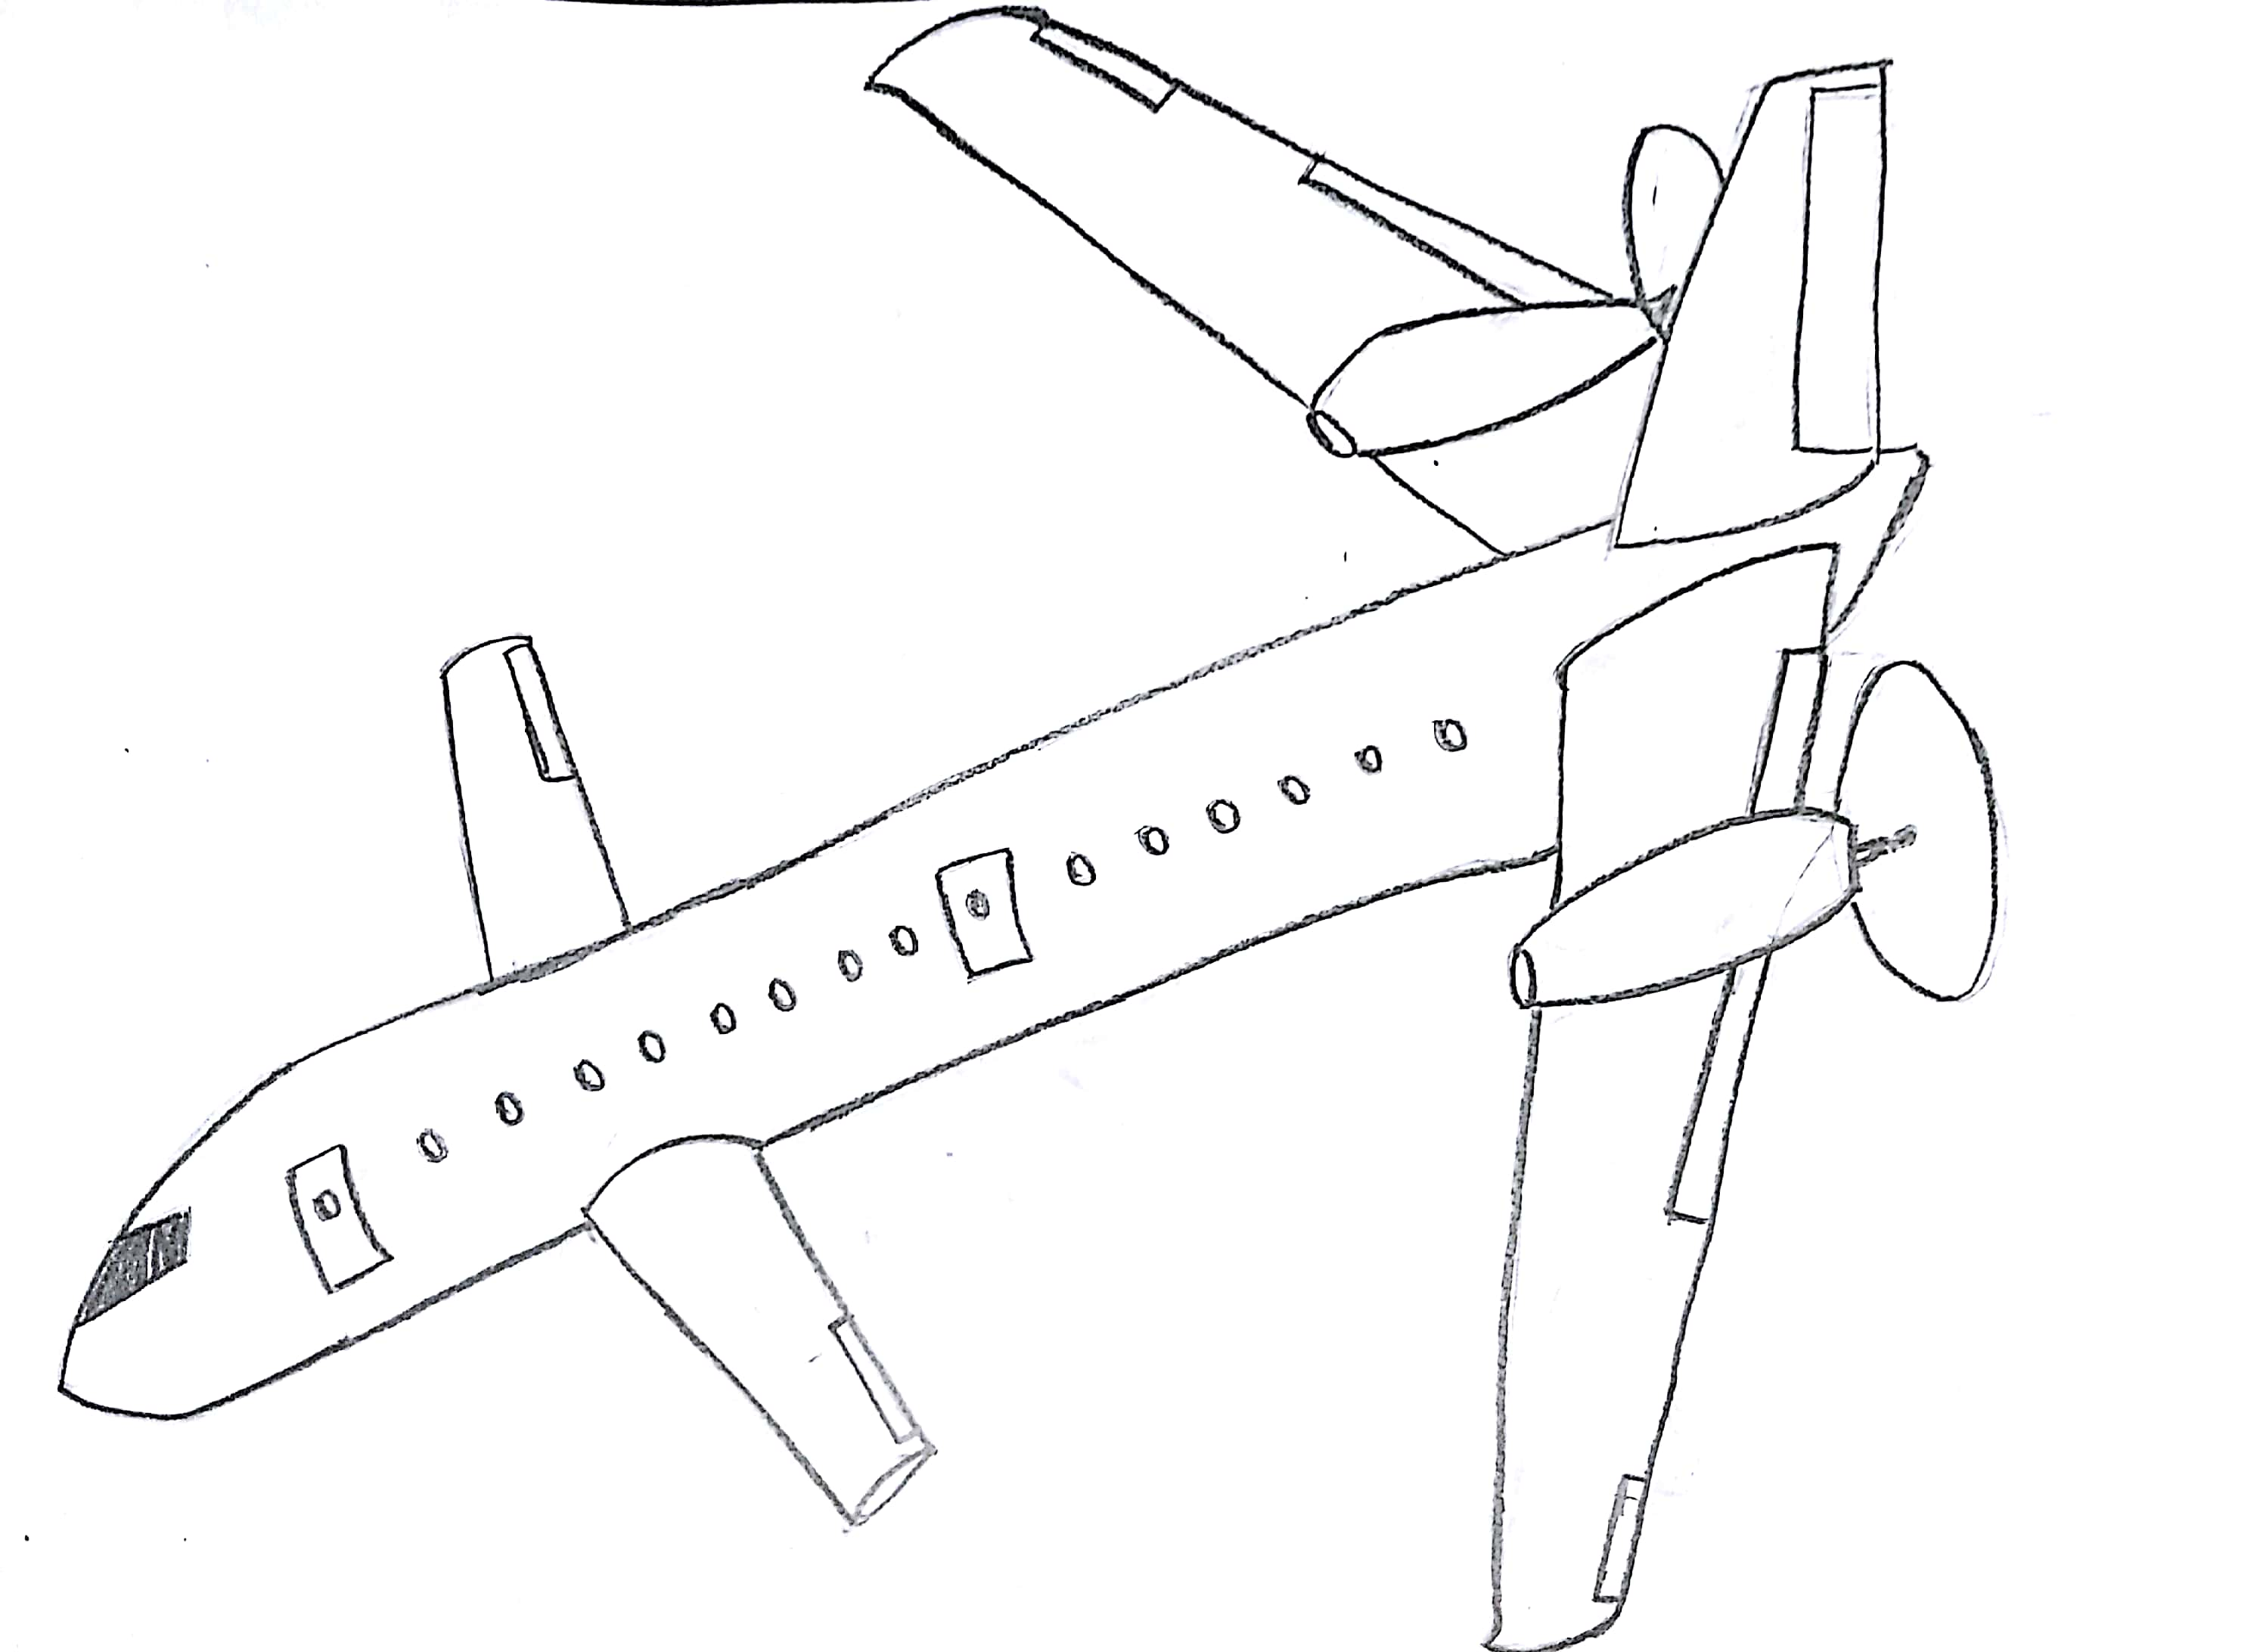
\includegraphics[width=0.6\textwidth,angle=0]{Modelos_Projetos_1_3.jpg}
\caption{Conceito de um turbo-hélice configuração \emph{canard}}
\label{fig:canard}
\end{figure}

Além disso, uma configuração em \emph{canard}, com motores turboprop em configuração \emph{pusher}, \autoref{fig:canard}, foi brevemente considerada, devido à segurança adicional de colocar o plano das hélices fora da cabine de passageiros.
Essa configuração foi considerada inviável porque as asas teriam que ficar demasiadamente para trás para não reduzir o espaço da cabine de passageiros, o que gera problemas de posicionamento do trem de pouso: colocá-lo longe das longarinas implica em um aumento de peso estrutural significativo, e colocá-lo demasiadamente a montante dificultaria a arfagem da aeronave durante a decolagem.
Além disso, o desempenho para pouso de aeronaves com configuração \emph{canard} é substancialmente pior do que as convencionais, devido ao fato de que, para manter a segurança do voo, aquele tipo de aeronave tem que voar substancialmente acima da velocidade de estol.

Com os avanços recentes na tecnologia de manufatura de materiais compostos, tornou-se viável a fabricação de aeronaves predominantemente feitas com estes materiais, como é o caso do Boeing~787 e Airbus~A350~XWB, ambos com 50\% ou mais do peso estrutural em materiais compostos.
De acordo com os fabricantes, isso levou a uma redução de aproximadamente 20\% no peso vazio da aeronave e de até 25\% nos custos operacionais.\cite{boeing:787,airbus:a350xwb}

Desta forma, a aeronave deste trabalho terá sua estrutura feita majoritariamente de materiais compostos, em especial fibra de carbono.
A aeronave da segunda opção, com enflechamento negativo, seria especialmente beneficiada, já que o uso de materiais compostos permite a adoção do conceito de \emph{aeroelastic tayloring}, que elimina o divergente aeroelástico característico de asas enflechadas negativamente.
Esse tipo de construção tem vantagens aerodinâmicas como atraso do estol, em especial nas pontas de asa, o que faz a aeronave mais controlável a baixas velocidades, e portanto aumenta a segurança do pouso ou, mantendo a segurança, permite o uso de menos superfícies hipersustentadoras, o que justifica sua adoção em detrimento do enflechamento positivo, mais usual.\cite{weisshaar1980forward}

Além disso, o uso de motores propfan em vez de turbofan pode reduzir o consumo da aeronave em até 30\%\cite{safran:propfan}. 
O maior problema desse tipo de motor é o ruído, mas isso pode ser mitigado por uma solução similar a \cite{emmanuel2009patent}, na qual o motor fica entre as duas empenagens verticais.
O simples avanço tecnológico também pode resolver esse problema\cite{ge:propfan}.
Um projeto de propfan está disponível em \cite{nasa:propfan}.

Em relação à primeira configuração, os ganhos de desempenho em relação aos competidores viriam do menor peso vazio possível devido ao uso de compósitos e aos avanços tecnológicos nos motores.

\subsection{Ergonomia Interna}

Para definição inicial da ergonomia interna, decidiu-se avaliar os dois principais concorrentes no segmento analisado na pesquisa de mercado: CRJ200 e ERJ-145.
Estas duas aeronaves apresentam configurações de \textit{cross-section} e LOPA (\textit{Layout Of Passenger Accommodation}) distintas.
A aeronave CRJ200 tem quatro poltronas por fileira e 13 fileiras no total.
Já a aeronave ERJ-145 tem três poltronas por fileira e 16 fileiras no total.
Para aproximadamente um mesmo número de passageiros, um número maior de poltronas por fileiras implica em uma fuselagem com um comprimento menor e um diâmetro da seção maior.
Abaixo, tem-se uma tabela que resume as dimensões externas referentes à fuselagem e à configuração interna para cada avião:

\begin{table}[H]
\centering
\begin{tabular}{cccccc}
\toprule
Aeronaves & Passageiros & N\textdegree\  de Poltronas  & N\textdegree\  de Fileiras & Comprimento & Diâmetro \\
	&	&por Fileiras	&	& (m) & (m) \\ \midrule
CRJ200 & 50 & 4 & 13 & 26.77 & 2.5 \\
ERJ145 & 48 & 3 & 16 & 29.87 & 2.1 \\
\bottomrule
\end{tabular}

\caption[Dimensões da Fuselagem]{Dados referentes à fuselagem e à configuração interna das aeronaves CRJ200 E ERJ145.}
\label{tbl:comparacao_fus}
\end{table}

A distribuição interna dos passageiros implica diretamente nas dimensões da fuselagem.
Por sua vez, a geometria da fuselagem implica, principalmente, em dois parâmetros: 

\begin{enumerate}
	\item Contribuição da fuselagem no arrasto total da aeronave
	\item Peso vazio total
\end{enumerate}

Para análises preliminares das duas aeronaves em discussão em termos de arrasto da fuselagem, utilizou-se a referência \cite{nasatn6800}.
O coeficiente de arrasto da fuselagem é definido pela equação abaixo:

\begin{equation}
C_{D_{0_f}} = C_f f_{ld} f_M \frac{S_{wet_{fus}}}{S}
\end{equation}

Em que:

\begin{equation}
C_{f} = \frac{0.455}{\log{Re^{2.58}}}
\end{equation}

\begin{equation}
f_{ld} =  1 + 60/(\frac{l}{d})^3 + 0.0025(\frac{l}{d})
\end{equation}

\begin{equation}
f_{M} = 1- 0.08M^{1.45}
\end{equation}

\begin{equation}
S_{wet_{fus}} = \pi d l 
\end{equation}

\begin{description}
 \item[$S_{wet_{fus}}$ -]área molhada da fuselagem considerando aproximação para cilindro
 \item[$S$ -]área de referência da asa
 \item[$C_f$ -]coeficiente de fricção do revestimento para escoamento turbulento
 \item[$f_M$ -]fator em função do número de Mach
 \item[$f_{ld}$ -]fator em função do comprimento e diâmetro da fuselagem
 \item[$Re$ -]número de Reynolds
 \item[$M$ -]número de Mach
 \item[$l$ -]comprimento da fuselagem
 \item[$d$ -]diâmetro da fuselagem
\end{description}

Considerando que os termos $Cf$, $f_M$ e $S$ são iguais para ambas as aeronaves para fins de análise, pode-se avaliar o impacto da geometria externa da fuselagem a partir dos termos $f_{ld}$ e $S_{wet_{fus}}$.
Dessa forma, tem-se a estimativa abaixo para o avião CRJ200 e ERJ145 a partir da expressão

\begin{equation}
Impacto_{C_D} = \frac{C_{D_{0_f}}}{ C_f f_M /S  } = f_{ld} S_{wet_{fus}}
\end{equation}

\begin{table}[H]
\centering
\begin{tabular}{cccc}
\toprule
Aeronave & $S_{wet_{fus}}$ & $f_{ld}$ & $Impacto_{C_D}$ \\ \midrule
CRJ200 & 209 & 1.075 & 224 \\
ERJ145 & 197 & 1.056 & 208 \\
\bottomrule
\end{tabular}
\caption[Arrasto da Fuselagem]{Impacto da geometria da fuselagem no seu arrasto}
\label{tbl:impacto_fus}
\end{table}

A partir dos resultados acima, pode-se observar que a fuselagem da aeronave CRJ200 tem um arrasto estimado $8\%$ maior. A prioridade deste trabalho é projetar uma aeronave com baixo consumo de combustível, logo, a partir da análise dos concorrentes, um fuselagem maior em comprimento permite uma redução do arrasto. Nesta primeira análise, portanto, estabeleceu-se que uma configuração com três poltronas por fileira é uma opção mais competitiva.

Outro impacto da geometria da fuselagem é em relação ao tamanho das empenagens. Caso a fuselagem seja maior em comprimento, para um mesmo momento no CG da aeronave, a força resultante das empenagens deve ser menor visto que o braço é maior. Logo, as empenagens podem ter uma área menor, o que reduz diretamente o arrasto, visto que

\begin{equation}
D_{empenagens} =  0.5 \rho V^2 S_{EH} C_{D_{EH}} + 0.5 \rho V^2 S_{EV} C_{D_{EV}}  
\end{equation}

\begin{description}
	\item[$S_{EV}$ -]área em planta da empenagem vertical
    \item[$S_{EH}$ -]área em planta da empenagem horizontal
\end{description}


Além disso, empenagens com áreas menores implicam em uma redução no peso vazio do conjunto.
O impacto da redução do peso vazio pode ser analisado em termos de arrasto.
No caso, sabe-se que uma parcela do arrasto é o arrasto induzido que é função da sustentação.
Em voo reto e nivelado, a sustentação deve equilibrar o peso da aeronave, logo, um peso total menor devido a uma redução em peso vazio implica em uma menor sustentação necessária.
O que por sua vez implica em um menor arrasto induzido e dessa forma uma redução no arrasto em cruzeiro. 
Portanto, tem-se um terceiro benefício ao se optar por três poltronas por fileira visto que uma fuselagem maior em comprimento reduz o arrasto de trimagem das empenagens em cruzeiro.

Sobre o impacto no peso vazio da fuselagem devido a sua geometria, sabe-se que uma fuselagem maior em comprimento apresenta um diâmetro menor. Em relação à estrutura da fuselagem, considera-se para fins de análise que a carga integrada na seção média de ambas as aeronaves é igual. Além disso, tem-se a seguinte equação para tensão normal devido ao momento de flexão na seção de análise

\begin{equation}
\sigma =  \frac{M y }{I} 
\end{equation}
\begin{equation}
I =  \frac{\pi(D^4 - (D-t)^4)}{64}
\end{equation}

\begin{description}
	\item[$\sigma$ -] tensão normal devido ao momento de flexão
    \item[$M$ -] Momento de flexão na seção média da fuselagem
    \item[$y$ -] distância em relação ao centroide da seção, no caso de um cilindro oco simétrico, $y_{max} = \frac{d}{2}$
    \item[$I$ -] momento de inércia para um cilindro oco
    \item[$t$ -] espessura do revestimento da fuselagem
    \item[$D$ -] diâmetro externo da fuselagem
\end{description}

Considerando que o comportamento da estrutura da fuselagem pode ser aproximado para equação acima, tem-se que a tensão normal deve ser menor que a tensão admissível do material utilizado.
Além disso, considera-se também que ambas as aeronaves utilizam o mesmo material na estrutura da fuselagem.

Como pode ser observado na equação, uma fuselagem maior em comprimento e menor em diâmetro tem uma redução na parcela do momento de inércia que é função do diâmetro externo somente.
Dessa forma, visto que o momento de flexão é mesmo em ambas as fuselagens, o momento de inércia deve permanecer o mesmo para ainda atender a condição de que a tensão normal atuante na fuselagem deve ser menor que a tensão admissível do material.
Logo, para evitar uma redução no momento de inércia, deve-se aumentar a espessura do revestimento da fuselagem o que implica em um aumento em peso vazio no caso da fuselagem maior em comprimento e menor em diâmetro.
O impacto do aumento no peso vazio da fuselagem segue o mesmo raciocínio apresentado para a redução do peso vazio do conjuto de empenagens.
Portanto, este fato é um ponto negativo para a fuselagem maior em comprimento com três poltronas por fileira. 

A partir das discussões acimas, pode-se resumir os impactos analisados na lista abaixo para a configuração com três poltronas por fileira

\begin{enumerate}
	\item Redução no arrasto da fuselagem 
    \item Redução no arrasto do conjunto de empenagens
    \item Redução no peso vazio do conjunto de empenagens
    \item Aumento no peso vazio da fuselagem
\end{enumerate}

Dessa forma, tem-se três pontos positivos e um negativo para a configuração com três poltronas por fileira.
O contrário se aplica para a configuração interna com quatro poltronas por fileira.
O questionamento associado a esses aspectos discutidos para a primeira distribuição de passageiros é se o aumento no peso vazio da fuselagem sobrepõe os outros três benefícios apresentados.
De forma a concluir sobre o aspecto de peso, tem-se abaixo uma tabela que compara o peso vazio de ambas as aeronaves.

\begin{table}[H]
\centering
\begin{tabular}{cc}
\toprule
Aeronave & Peso Vazio (kg) \\ \midrule
CRJ200 & 13835 \\
ERJ145 & 12114 \\
\bottomrule
\end{tabular}
\caption[Peso Vazio das Aeronaves em Análise]{Peso vazio para as aeronaves CRJ200 e ERJ145}
\label{tbl:pesovazio_fus}
\end{table}

Como pode ser observado, apesar de uma fuselagem maior em comprimento implicar em uma fuselagem mais pesada, a aeronave ERJ145 tem um peso vazio menor.
A redução no peso vazio das empenagens e outras soluções de projeto para otimização das estruturas para uma aeronave com fuselagem maior em comprimento sobrepõem o ponto negativo desta configuração viabilizando a configuração interna com três poltronas por fileira.

Portanto, conclui-se que uma configuração com três poltronas por fileira oferece menor arrasto em cruzeiro e menor peso vazio.
Logo, esta geometria é mais competitiva e permite um menor consumo de combustível.
Abaixo tem-se a idealização da configuração interna da aeronave a ser projetada com três poltronas por fileira. 

\begin{figure}[p]
\centering
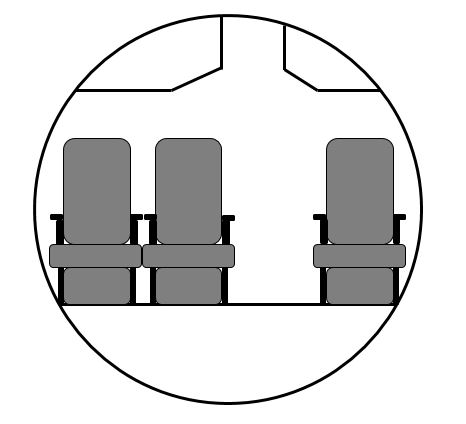
\includegraphics[width=0.5\textwidth]{CrossSectionPRJ1.JPG}
\caption{Seção transversal da aeronave em projeto}
\end{figure}

\begin{figure}[p]
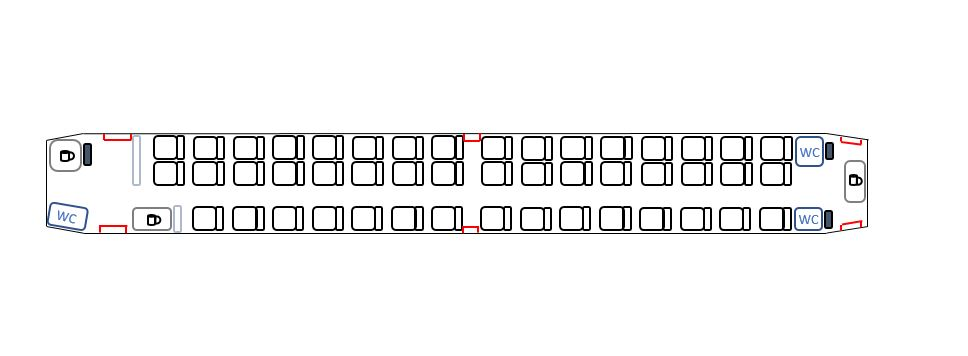
\includegraphics[width=\textwidth]{LopaPRJ1.JPG}
\caption{Seção longitudinal da aeronave em projeto}
\end{figure}
